

\chapter{Interpolação}\label{cap_interp}
\thispagestyle{fancy}

Neste capítulo, discutiremos sobre a resolução de problemas de interpolação da forma: dados uma família de $n$ funções reais $\mathcal{F} = \{f_1(x), f_2(x), \ldots, f_n(x)\}$ e um conjunto de $n$ pontos $\{(x_i, y_i)\}_{i=1}^n$, com $x_i\neq x_j$ se $i\neq j$, encontrar
\begin{equation}
  f(x) = c_1f_1(x) + c_2f_2(x) + \cdots + c_nf_n(x),
\end{equation}
tal que
\begin{equation}
  y_i = f(x_i),\quad i=1, 2, \ldots, n.
\end{equation}

\section{Interpolação polinomial}\label{cap_interp_sec_interpoli}

Dado um conjunto de $n$ pontos $\{(x_i, y_i)\}_{i=1}^n$, o problema de interpolação consiste em encontrar o polinômio de grau $n-1$
\begin{equation}\label{eq:interpoli_poli}
  p(x) = p_1x^{n-1} + p_2x^{n-2} + \cdots + p_{n-1}x + p_n
\end{equation}
tal que
\begin{equation}\label{eq:interpoli_conds}
  y_i = p(x_i),\quad i=1, 2, \ldots, n.
\end{equation}

Das condições \eqref{eq:interpoli_poli}, temos
\begin{align}\label{eq:interpoli_sis}
  p_1x_1^{n-1} + p_2x_1^{n-2} + \cdots + p_{n-1}x_1 + p_n &= y_1 \\
  p_1x_2^{n-1} + p_2x_2^{n-2} + \cdots + p_{n-1}x_2 + p_n &= y_2 \\
  &\vdots \\
  p_1x_n^{n-1} + p_2x_n^{n-2} + \cdots + p_{n-1}x_n + p_n &= y_n.
\end{align}
Isto é, os coeficientes do polinômio interpolador \eqref{eq:interpoli_poli} satisfazem o seguinte sistema linear
\begin{equation}
  A\pmb{p} = \pmb{y},
\end{equation}
onde $A$ é a matriz de Vandermonde\footnote{Alexandre-Théophile Vandermonde, 1735 - 1796, matemático francês. Fonte: \href{https://en.wikipedia.org/wiki/Alexandre-Th\%C3\%A9ophile_Vandermonde}{Wikipedia}.}
\begin{equation}
  A =
  \begin{bmatrix}
    x_1^{n-1} & x_1^{n-2} & \ldots & x_1 & 1 \\
    x_2^{n-1} & x_2^{n-2} & \ldots & x_2 & 1 \\
    \vdots  & \vdots  & \vdots  & \vdots & \vdots \\
    x_n^{n-1} & x_n^{n-2} & \ldots & x_n & 1
  \end{bmatrix},
\end{equation}
$\pmb{p} = (p_1, p_2, \ldots, p_n)$ é o vetor das incógnitas e $\pmb{y} = (y_1, y_2, \ldots, y_n)$ é o vetor dos termos constantes.

\begin{ex}\label{ex:interpoli_intro}
  Consideremos o problema de encontrar o polinômio interpolador do conjunto de pontos $\{(-1,~-1), (0,~1), (1,~1/2)\}$. Como temos 3 pontos, o polinômio tem grau 2 e pode ser escrito na forma
  \begin{equation}
    p(x) = p_1x^2 + p_2x + p_3.
  \end{equation}
  Seguindo a abordagem acima, temos $\pmb{p}=(p_1, p_2, p_3)$, $\pmb{x} = (-1, 0, 1)$, $\pmb{y}=(-1, 1, 1/2)$ e
  \begin{equation}
    A =
    \begin{bmatrix}
      x_1^2 & x_1 & 1\\
      x_2^2 & x_2 & 1\\
      x_3^2 & x_3 & 1
    \end{bmatrix}.
  \end{equation}
  Então, resolvendo $A\pmb{p} = \pmb{y}$, obtemos o polinômio interpolador
  \begin{equation}
    p(x) = -1,25x^2 + 0,75x + 1.
  \end{equation}
A Figura \ref{fig:interpoli_intro} mostra os esboços do polinômio interpolador $p(x)$ e  dos pontos dados.

\begin{figure}[h!]
  \centering
  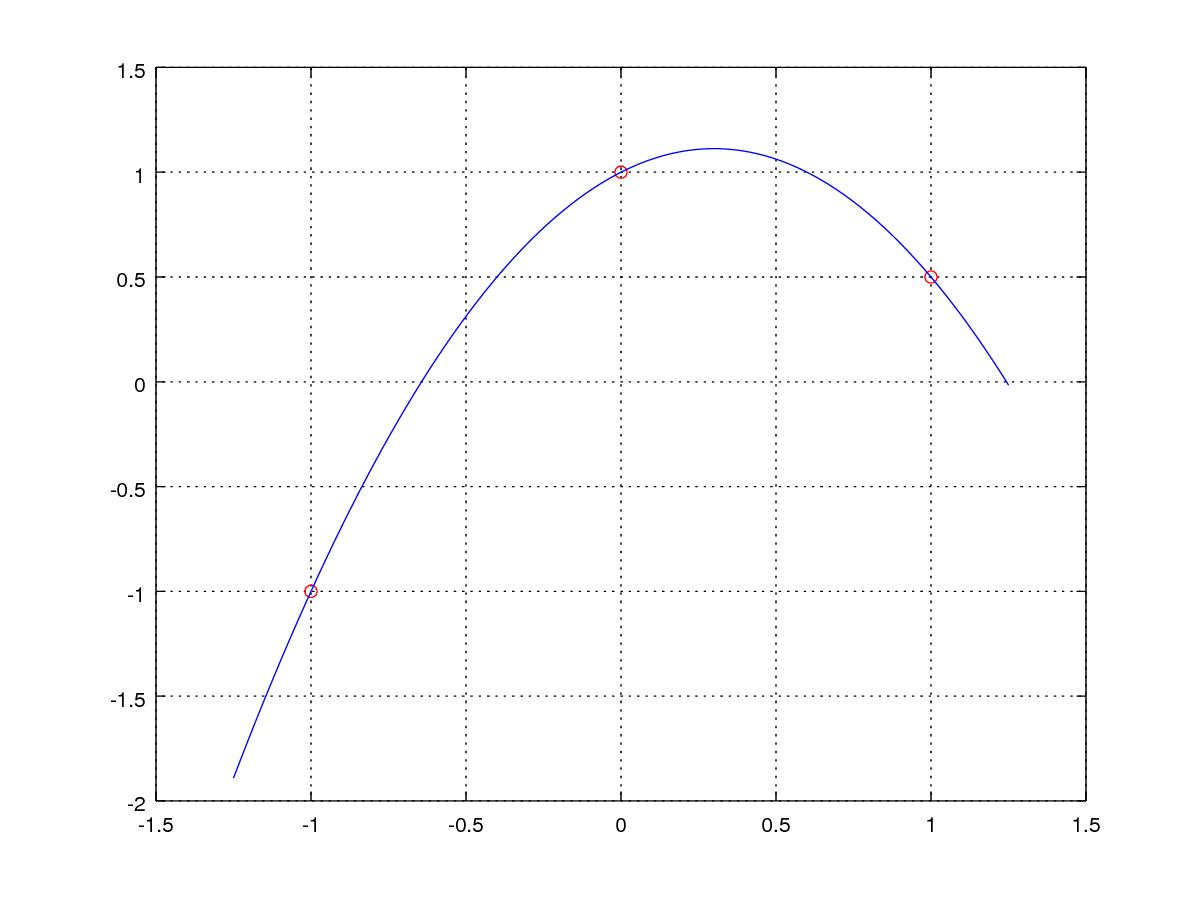
\includegraphics[width=0.7\textwidth]{./cap_interp/dados/ex_interpoli_intro/fig_interpoli_intro}
  \caption{Esboços dos pontos e do polinômio interpolador referente ao Exemplo \ref{ex:interpoli_intro}.}
  \label{fig:interpoli_intro}
\end{figure}

% \ifisoctave
% No \verb+GNU Octave+, podemos fazer as computações acima com o seguinte \href{https://github.com/phkonzen/notas/blob/master/src/MatematicaNumerica/cap_interp/dados/ex_interpoli_intro/ex_interpoli_intro.m}{código}:
% \verbatiminput{./cap_interp/dados/ex_interpoli_intro/ex_interpoli_intro.m}
% \fi
\end{ex}

\subsection*{Exercícios}

\begin{exer}\label{exer:interpoli_intro1}
  Obtenha o polinômio interpolador do conjunto de pontos $\{(-1,~-1), (0,~1), (1,~1/2), (2,~1)\}$.
\end{exer}
\begin{resp}
% \ifisoctave
% \href{https://github.com/phkonzen/notas/blob/master/src/MatematicaNumerica/cap_interp/dados/exer_interpoli_intro1/exer_interpoli_intro1.m}{Código}.
% \fi
$0,58\bar{3}x^2 - 1,25x + 0,1\bar{6} + 1$.  
\end{resp}

\emconstrucao

\section{Interpolação de Lagrange}\label{cap_interp_sec_lagrange}

Interpolação de Lagrange\footnote{Joseph-Louis Lagrange, 1736 - 1813, matemático italiano. Fonte: \href{https://en.wikipedia.org/wiki/Joseph-Louis_Lagrange}{Wikipedia}.} é uma técnica para a computação do polinômio interpolador $p(x)$ de um conjunto de pontos $\{(x_i, y_i)\}_{i=1}^n$ dados. A ideia consiste em escrever o polinômio interpolador na forma
\begin{equation}
  p(x) = y_1L_1(x) + y_2L_2(x) + \cdots + y_nL_n(x),
\end{equation}
onde $L_i(x)$ é chamado de $i$-ésimo polinômio de Lagrange e é definido como o polinômio de grau $n-1$ que satisfaz
\begin{equation}
  L_i(x_j) = \left\{
    \begin{array}{ll}
      1 &, i=j\\
      0 &, i\neq j
    \end{array}
\right.
\end{equation}
Mais especificamente, temos que $L_i(x)$ tem raízes $\{x_1, \ldots, x_{i-1}, x_{i+1}, \ldots, x_n\}$ e, portanto, pode ser decomposto na forma
\begin{equation}
  L_i(x) = c_i(x-x_1)\cdots(x-x_{i-1})(x-x_i)\cdots(x-x_n).
\end{equation}
Além disso, como $L_i(x_i) = 1$, temos
\begin{equation}
  c_i = \frac{1}{(x_i-x_1)\cdots(x_i-x_{i-1})(x_i-x_i)\cdots(x_i-x_n)}.
\end{equation}
Assim sendo, podemos concluir que
\begin{equation}
  L_i(x) = \frac{(x-x_1)\cdots(x-x_{i-1})(x-x_{i+1})\cdots(x-x_n)}{(x_i-x_1)\cdots(x_i-x_{i-1})(x_i-x_{i+1})\cdots(x_i-x_n)}.
\end{equation}


\begin{ex}
  Consideremos o problema de encontrar o polinômio interpolador do conjunto de pontos $\{(-1,~-1), (0,~1), (1,~1/2)\}$. Como temos 3 pontos, o polinômio tem grau 2 e pode ser escrito na seguinte forma de Lagrange
  \begin{equation}
    p(x) = y_1L_1(x) + y_2L_2(x) + y_3L_3(x),
  \end{equation}
  onde $y_1 = -1$, $y_2 = 1$ e $y_3 = 1/2$. Os polinômios de Lagrange são dados por
  \begin{align}
    L_1(x) &= \frac{(x-x_2)(x-x_3)}{(x_1-x_2)(x_1-x_3)} = \frac{1}{2}x^2 - \frac{1}{2}x,\\
    L_2(x) &= \frac{(x-x_1)(x-x_3)}{(x_2-x_1)(x_2-x_3)} = -x^2 + 1,\\
    L_3(x) &= \frac{(x-x_1)(x-x_2)}{(x_3-x_1)(x_3-x_2)} = \frac{1}{2}x^2 + \frac{1}{2}x.\\
  \end{align}
  E, então, temos o polinômio interpolador
  \begin{equation}
    p(x) = -1,25x^2 + 0,75x + 1.
  \end{equation}

% \ifisoctave
% No \verb+GNU Octave+, podemos fazer as computações acima com o seguinte \href{https://github.com/phkonzen/notas/blob/master/src/MatematicaNumerica/cap_interp/dados/ex_interpoli_lagrange/ex_interpoli_lagrange.m}{código}:
% \verbatiminput{./cap_interp/dados/ex_interpoli_lagrange/ex_interpoli_lagrange.m}
% \fi
\end{ex}

\subsection{Aproximação de funções}

Polinômio interpoladores podem ser usados para a aproximação de funções. Podemos aproximar uma dada função $f$ pelo polinômio interpolador de um conjunto de pontos selecionados $\{(x_i, y_i=f(x_i))\}_{i=1}^n$. De fato, o seguinte teorema nos fornece uma estimativa para o erro de uma tal interpolação.

\begin{teo}(\normalfont{\hl{Teorema de Lagrange}.})\label{cap_interp_sec_lagrange:teo:lagrange}
  Sejam dados uma função $f$ $n+1$-vezes continuamente diferenciável em um dado intervalo $[a, b]$ e $n$ pontos $\{x_i\}_{i=1}^n\subset [a, b]$. Então, o polinômio interpolador do conjunto de pontos $\{x_i, y_i=f(x_i)\}_{i=1}^n$ satisfaz
  \begin{equation}
    f(x) = p(x) + \frac{f^{(n+1)}(\xi)}{(n+1)!}(x-x_1)(x-x_2)\cdots (x-x_n).
  \end{equation}
\end{teo}
\begin{dem}
  \emconstrucao
\end{dem}

\begin{ex}\label{ex:interpoli_aprox}
  Considere o problema de aproxima $f(x) = \sen(x)$ pelo polinômio interpolador pelo conjunto de pontos $x_1=0$, $x_2=\pi/2$ e $x_3=\pi$. Isto, queremos determinar o polinômio $p(x)$ de grau $2$ que interpola os pontos $\{(0,0),~(\pi/2,~1),~(\pi,0)\}$. Usando a técnica de Lagrange, obtemos
  \begin{equation}
    p(x) = -0,41x^2 + 1,3x,
  \end{equation}
com seus coeficientes arredondados para dois dígitos significativos. A Figura \ref{fig:interpoli_aprox} mostra os esboços da função $f(x)=\sen(x)$, dos pontos dados e do polinômio interpolador $p(x)$.

\begin{figure}[h!]
  \centering
  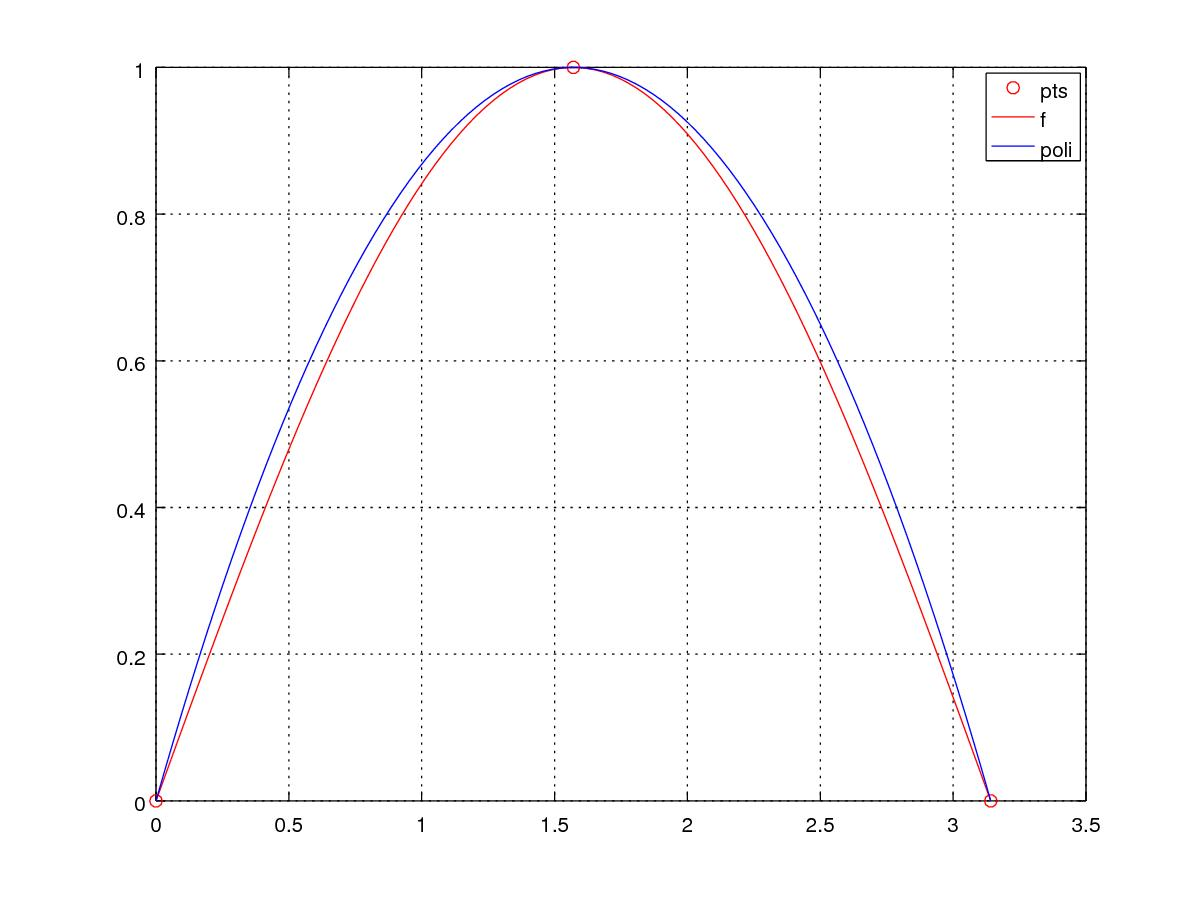
\includegraphics[width=0.7\textwidth]{./cap_interp/dados/ex_interpoli_aprox/fig_interpoli_aprox}
  \caption{Esboços dos gráficos da função, dos pontos e do polinômio interpolador computado no Exemplo \ref{ex:interpoli_aprox}.}
  \label{fig:interpoli_aprox}
\end{figure}

% \ifisoctave
% No \verb+GNU Octave+, podemos fazer as computações acima com o seguinte \href{https://github.com/phkonzen/notas/blob/master/src/MatematicaNumerica/cap_interp/dados/ex_interpoli_aprox/ex_interpoli_aprox.m}{código}:
% \verbatiminput{./cap_interp/dados/ex_interpoli_aprox/ex_interpoli_aprox.m}
% \fi
\end{ex}

\subsection*{Exercícios}

\begin{exer}
  Use a técnica de interpolação de Lagrange para encontrar o polinômio interpolador que aproxima a função$f(x)=e^{x}$ pelos pontos $x_1=0$, $x_2=1$, $x_3=1,5$ e $x_4=2$.
\end{exer}
\begin{resp}
% \ifisoctave
% \href{https://github.com/phkonzen/notas/blob/master/src/MatematicaNumerica/cap_interp/dados/exer_interpoli_aprox1/exer_interpoli_aprox1.m}{Código}.
% \fi
$0,54x^3 - 0,15x^2 + 1,3x + 1$.
\end{resp}

\emconstrucao

\section{Diferenças divididas de Newton}\label{cap_interp_difdiv}

Dado um conjunto de pontos $\{(x_i, y_i)\}_{i=1}^n$, o método das diferenças divididas de Newton\footnote{Carl Gustav Jacob Jacobi, 1804 - 1851, matemático alemão. Fonte: \href{https://en.wikipedia.org/wiki/Carl_Gustav_Jacob_Jacobi}{Wikipedia}.} busca determinar o polinômio interpolar deste conjunto de pontos na forma
\begin{align}
  p(x) &= a_1 + a_2(x-x_1) + a_3(x-x_1)(x-x_2)\\
       &+ \cdots + a_{n}(x-x_1)\cdot \cdots \cdot (x-x_{n-1}).
\end{align}

Por uma abordagem direta, temos que $p(x_i)=y_i$, $i=1, 2, \dotsc, n$, o que nos leva ao seguinte sistema triangular inferior
\begin{align}
  a_1 &= y_1, \\
  a_1 + a_2(x_2-x_1) &= y_2, \\
  a_1 + a_2(x_3-x_1) + a_3(x_3-x_1)(x_3-x_2) &= y_3, \\
  &\vdots\\
  a_1 + a_2(x_n-x_1) + \cdots + a_{n}(x_n-x_1)\cdot\cdots\cdot(x_n-x_{n-1}) &= y_n.
\end{align}
Entretanto, existe uma forma mais eficiente de se determinar os coeficientes $a_i$, $i=1, 2, \dotsc, n$.

Denotemos por $p[x_j, x_{j+1}, \dotsc, x_{k}](x)$ o polinômio interpolador do conjunto de pontos $\{(x_i, y_i)\}_{i=j}^k$. Então, temos a seguinte recursão
\begin{equation} \label{eq:interp_parc1}
  p[x_j] = y_j,\quad j=1, 2, \dotsc, n,
\end{equation}
e
\begin{align}
  &p[x_j, x_{j+1}, \ldots, x_k](x) \nonumber\\
  &= \frac{(x-x_j)p[x_{j+1},\dotsc,x_k](x)-(x-x_k)p[x_j,\dotsc,x_{k-1}](x)}{x_k-x_j},\label{eq:interp_parc2}
\end{align}
para todo $n\geq k > j \geq 1$. De fato, \eqref{eq:interp_parc1} é trivial. Agora, denotando por $r(x)$ o lado direito da equação \eqref{eq:interp_parc2}, vemos que $r(x)$ tem grau menor ou igual a $k-j$, o mesmo de $p[x_j, x_{j+1}, \ldots, x_k](x)$. Desta forma, para mostrar \eqref{eq:interp_parc2}, basta verificarmos que $r(x)$ interpola o conjunto de pontos $\{(x_i, y_i)\}_{i=j}^k$. O que de fato ocorre:
\begin{align}
  r(x_j) &= \frac{-(x_j-x_k)y_j}{x_k-x_j} = y_j,\\
  r(x_{l}) &= \frac{(x_l-x_j)y_l-(x_l-x_k)y_l}{x_k-x_j}=y_l,~l=j+1,\dotsc,k-1,\\
  r(x_k) &= \frac{(x_k-x_j)y_k}{x_k-x_j}=y_k.
\end{align}
Logo, pela unicidade do polinômio interpolador, temos demonstrado \eqref{eq:interp_parc2}.

Observando que o polinômio interpolador $p(x)$ é igual a $p[x_1,\dotsc,x_n](x)$, temos que \eqref{eq:interp_parc1}-\eqref{eq:interp_parc2} nos fornece uma forma de computar $p(x)$ recursivamente\footnote{De fato, o método de Neville consistem em computar $p(x)$ por esta recursão.}. Além disso, observemos que $p[x_j,\dotsc,x_{k-1}](x)$ e $p[x_j,\dotsc,x_k]$ diferem por um polinômio de grau $k-j$ com zeros $x_j$, $x_{j+1}$, ..., $x_{k-1}$. Logo, temos
\begin{align}
  p[x_j,\dotsc,x_k](x) &= p[x_j,\dotsc,x_{k-1}](x) \nonumber \\
                       &+ f[x_j,\dotsc,x_k](x-x_j)\cdot\cdots\cdot(x-x_{k-1}),
\end{align}
onde $f[x_j,\dotsc,x_k]$ são coeficientes a determinar. Ainda, tomando $p[x_i]=f[x_i]$, temos
\begin{align}
  p[x_j,\dotsc,x_k](x) &= f[x_j] + f[x_j,x_{j+1}](x-x_j) \nonumber \\
                       &+ f[x_j,\dotsc,x_k](x-x_j)\cdot\cdots\cdot(x-x_{k-1}).
\end{align}
Por fim, a recursão \eqref{eq:interp_parc1}-\eqref{eq:interp_parc2} nos mostra que as diferenças divididas Newton podem ser obtidas de
\begin{align}
  &f[x_j] = y_j,\quad j=1,2,\dotsc,n,\label{eq:interp_difdiv1}\\
  &f[x_j,\dotsc,x_k] = \frac{f[x_{j+1},\dotsc,x_k]-f[x_j,\dotsc,x_{k-1}]}{x_k-x_j},\label{eq:interp_difdiv2}
\end{align}
para todo $n\geq k>j\geq 1$. E, temos o polinômio interpolador do conjunto de pontos $\{(x_i,y_i)\}_{i=1}^n$ dado por
\begin{align}\label{eq:interpoli_Newton}
  p[x_1,\dotsc,x_n](x) &= f[x_1] + f[x_1,x_2](x-x_1) \nonumber \\
                       &+\cdots + f[x_1,\dotsc,x_n](x-x_1)\cdot\cdots\cdot(x-x_n).  
\end{align}

\begin{obs}
  A recursão \eqref{eq:interp_difdiv1}-\eqref{eq:interp_difdiv2} pode ser adequadamente organizada em uma matriz da forma
  \begin{equation}
    \begin{bmatrix}
      \pmb{f[x_1]} & 0 & 0 & \ldots & 0 \\
      f[x_2] & \pmb{f[x_1,x_2]} & 0 & \ldots & 0 \\
      f[x_3] & f[x_2,x_3] & \pmb{f[x_1,x_2,x_3]} & \ldots & 0\\
      \vdots & \vdots & \vdots & \ldots & \vdots \\
      f[x_n] & f[x_{n-1},x_{n}] & f[x_{n-2},x_{n-1},x_n] & \ldots & \pmb{f[x_1,x_2,\dotsc,x_n]}
    \end{bmatrix}
  \end{equation}
onde os elementos da diagonal correspondem aos coeficientes do polinômio interpolador na forma \eqref{eq:interpoli_Newton}.
\end{obs}


\begin{ex}
  Consideremos o problema de encontrar o polinômio interpolador do conjunto de pontos $\{(-1,~-1), (0,~1), (1,~1/2)\}$. Usando o método das diferenças divididas de Newton, escrevemos o polinômio na forma
  \begin{equation}
    p(x) = f[x_1] + f[x_1,x_2](x-x_1) + f[x_1,x_2,x_3](x-x_1)(x-x_2).
  \end{equation}
  Então, computamos seus coeficientes pela recursão \eqref{eq:interp_difdiv1}-\eqref{eq:interp_difdiv2}. Ou seja, temos
  \begin{equation}
    f[x_1]=-1,~f[x_2]=1,~f[x_3]=1/2.
  \end{equation}
  Daí, segue
  \begin{align}
    f[x_1,x_2] &= \frac{f[x_2]-f[x_1]}{x_2-x_1} = 2\\
    f[x_2,x_3] &= \frac{f[x_3]-f[x_2]}{x_3-x_2} = -\frac{1}{2}\\
  \end{align}
  e, então,
  \begin{equation}
    f[x_1,x_2,x_3] = \frac{f[x_2,x_3]-f[x_1,x_2]}{x_3-x_1}=-1,25.
  \end{equation}
  Logo, o polinômio interpolador é
  \begin{equation}
    p(x) = 0,5 + 2(x+1) - 1,25(x+1)(x-1),
  \end{equation}
  ou, equivalentemente,
  \begin{equation}
    p(x) = -1,25x^2 + 0,75x + 1.
  \end{equation}

% \ifisoctave
% No \verb+GNU Octave+, podemos fazer as computações acima com o seguinte \href{https://github.com/phkonzen/notas/blob/master/src/MatematicaNumerica/cap_interp/dados/ex_interpoli_difdiv/ex_interpoli_difdiv.m}{código}:
% \verbatiminput{./cap_interp/dados/ex_interpoli_difdiv/ex_interpoli_difdiv.m}
% \fi
\end{ex}

\subsection*{Exercícios}

\begin{exer}\label{exer_interpoli_difdiv1}
  Use o método das diferenças divididas de Newton para encontrar o polinômio interpolador que aproxima a função $f(x)=e^{x}$ pelos pontos $x_1=0$, $x_2=1$, $x_3=1,5$ e $x_4=2$.
\end{exer}
\begin{resp}
% \ifisoctave
% \href{https://github.com/phkonzen/notas/blob/master/src/MatematicaNumerica/cap_interp/dados/exer_interpoli_dfidiv1/exer_interpoli_difdiv1.m}{Código}.
% \fi
$0,54x^3 - 0,15x^2 + 1,3x + 1$.
\end{resp}

\emconstrucao

\section{Spline cúbico}\label{cap_interp_splines}

Dado um conjunto de pontos $\{(x_i,y_i)\}_{i=1}^n$, um spline cúbico é uma função duas vezes continuamente diferenciável da forma
\begin{equation}
  \begin{small}
    s(x)\!=\!\left\{
      \begin{array}{ll}
        \!s_{11}(x-x_1)^3 + s_{12}(x-x_1)^2 + s_{13}(x-x_1) + s_{14} &,x_1\!\leq\!x\!<\!x_2,\\
        \!s_{21}(x-x_2)^3 + s_{22}(x-x_2)^2 + s_{23}(x-x_2) + s_{24} &,x_2\!\leq\!x\!<\!x_3,\\
                                                                   &, \vdots \\
        \!s_{n-1,1}(x-x_2)^3\!+\!s_{n-1,2}(x-x_2)^2\!+\!s_{n-1,3}(x-x_2)\!+\!s_{n-1,4}\!&,x_{n-1}\!\leq\!x\!\leq\!x_n.
      \end{array}
    \right.
  \end{small}
\end{equation}
que satisfaz as seguintes propriedades
\begin{enumerate}
\item $s(x_i) = y_i$ para $i=1, 2, \dotsc, n$,
\item $s_j(x_j) = s_{j+1}(x_j)$ para todo $j=1,2,\dotsc,n-2$,
\item $s_j'(x_j) = s_{j+1}'(x_j)$ para todo $j=1,2,\dotsc,n-2$,  
\item $s_j''(x_j) = s_{j+1}''(x_j)$ para todo $j=1,2,\dotsc,n-2$.
\end{enumerate}

Observemos que o spline tem $4(n-1)$ coeficientes a determinar, enquanto que as condições acima nos fornecem $4n-6$ equações. Assim sendo, nota-se a determinação de um spline requer ainda 2 condições. Conforme a escolha destas condições, diferentes splines cúbicos são computados.

\subsection{Spline {\it Not-a-knot}}

A condição {\it not-a-knot} exige que o spline cúbico tenha derivada terceira contínua nos pontos $x_2$ e $x_{n-1}$, i.e.
\begin{equation}
  s_1'''(x_2) = s_2'''(x_2)\quad\text{e}\quad s_{n-2}'''(x_{n-1}) = s_{n-1}'''(x_{n-1}).
\end{equation}

\begin{ex}\label{ex:interp_spline_nak}
  Consideremos o problema de aproximar a função $f(x)=\sen(x)$ pelo spline cúbico {\it not-a-knot} com pontos suporte $x_1=0$, $x_2=\pi/3$, $x_3=\pi/6$ e $x_4=\pi/2$. Na Figura \ref{fig:interp_spline_nak} temos os esboços de $f$ e do spline cúbico computado.

  \begin{figure}[h!]
    \centering
    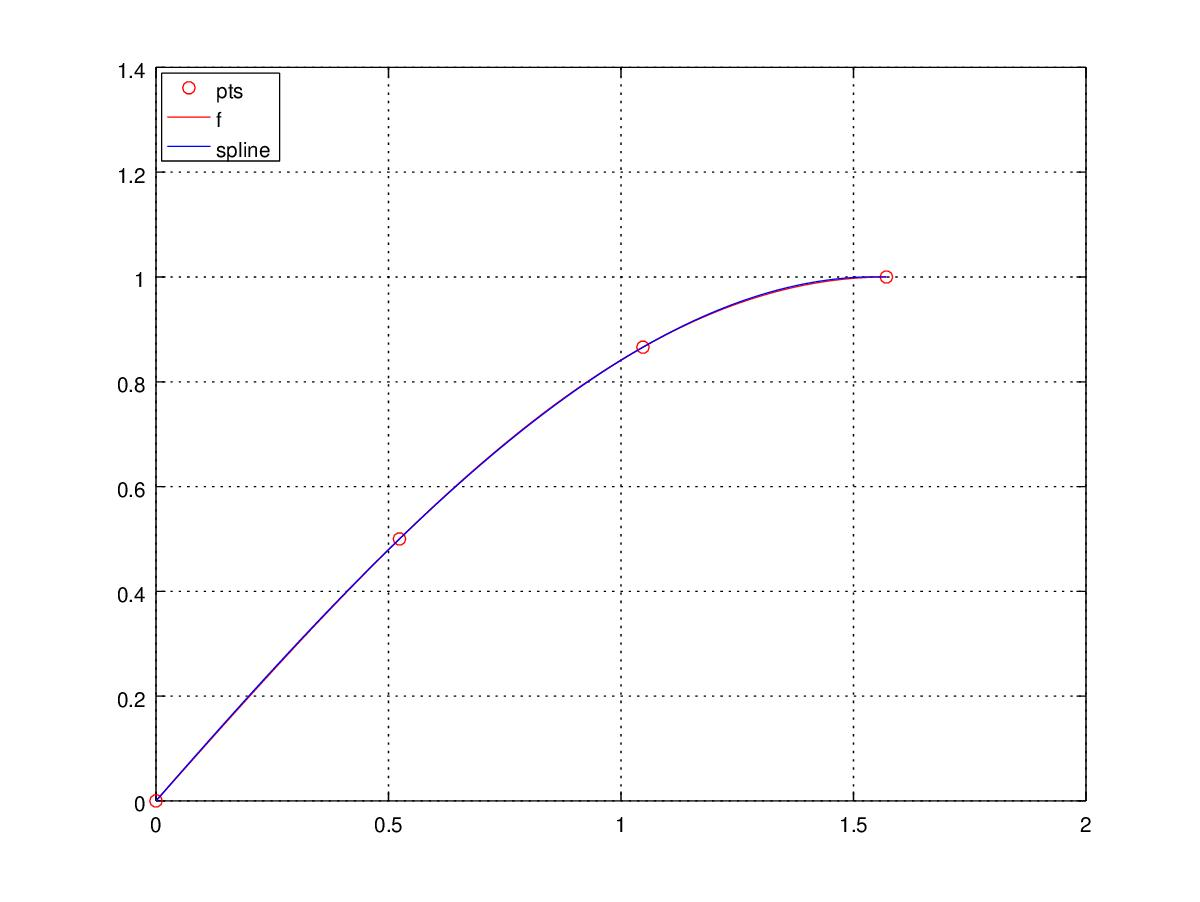
\includegraphics[width=0.7\textwidth]{./cap_interp/dados/ex_interp_spline_nak/fig_interp_spline_nak}
    \caption{Esboço dos gráficos da função $f(x)=\sen(x)$ e do spline cúbico computado no Exemplo \ref{ex:interp_spline_nak}.}
    \label{fig:interp_spline_nak}
  \end{figure}

% \ifisoctave
% No \verb+GNU Octave+, podemos fazer as computações acima com o seguinte \href{https://github.com/phkonzen/notas/blob/master/src/MatematicaNumerica/cap_interp/dados/ex_interp_spline_nak/ex_interp_spline_nak.m}{código}:
% \verbatiminput{./cap_interp/dados/ex_interp_spline_nak/ex_interp_spline_nak.m}
% \fi
\end{ex}

\subsection{Spline fixado}

Os splines cúbicos fixados são obtidos com as condições de fronteira
\begin{equation}
  s'(x_1)=y_1',\quad\text{e}\quad s'(x_n)=y_n',
\end{equation}
onde $y_1'$ e $y_n'$ são escalares dados. Quando usamos splines para aproximarmos uma dada função $f$, usualmente, escolhemos $y_1'=f'(x_1)$ e $y_n'=f'(x_n)$.

\begin{ex}\label{ex:interp_spline_fixado}
  Consideremos o problema de aproximar a função $f(x)=\sen(x)$ pelo spline cúbico fixado com pontos suporte $x_1=0$, $x_2=\pi/3$, $x_3=\pi/6$ e $x_4=\pi/2$. Na Figura \ref{fig:interp_spline_fixado} temos os esboços de $f$ e do spline cúbico computado.

  \begin{figure}[h!]
    \centering
    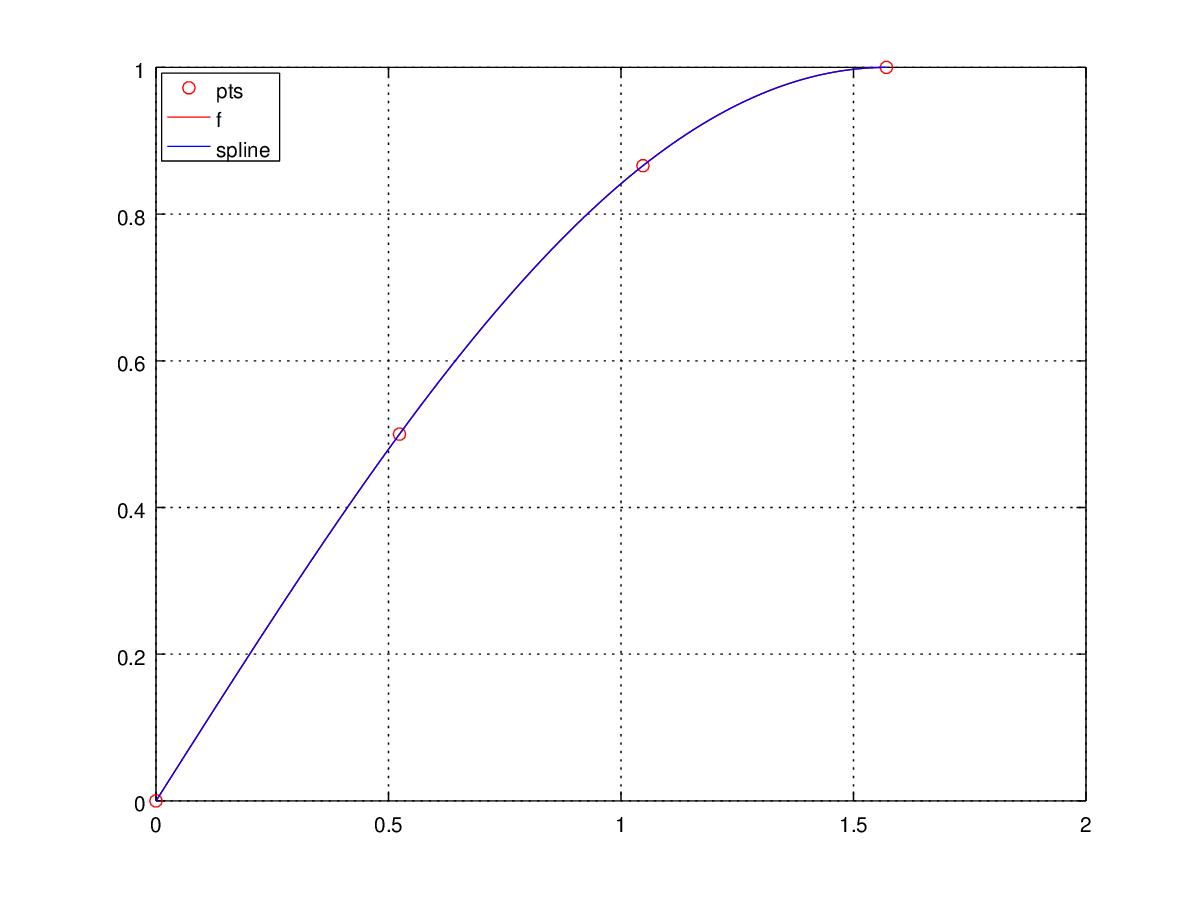
\includegraphics[width=0.7\textwidth]{./cap_interp/dados/ex_interp_spline_fixado/fig_interp_spline_fixado}
    \caption{Esboço dos gráficos da função $f(x)=\sen(x)$ e do spline cúbico computado no Exemplo \ref{ex:interp_spline_fixado}.}
    \label{fig:interp_spline_fixado}
  \end{figure}

% \ifisoctave
% No \verb+GNU Octave+, podemos fazer as computações acima com o seguinte \href{https://github.com/phkonzen/notas/blob/master/src/MatematicaNumerica/cap_interp/dados/ex_interp_spline_fixado/ex_interp_spline_fixado.m}{código}:
% \verbatiminput{./cap_interp/dados/ex_interp_spline_fixado/ex_interp_spline_fixado.m}
% \fi
\end{ex}

\subsection*{Exercícios}

\emconstrucao
